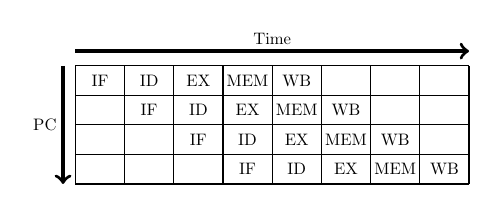
\begin{tikzpicture}[
		xscale=0.625,
		yscale=0.375,
		every node/.style={
			scale=0.6
		}
	]
	% Diagram
	\draw (1, 0) grid (9, -4);
	\foreach \i in {1,2,3,4} {
		\node at ({\i+0.5}, {0.5-\i}) {IF};
		\node at ({\i+1.5}, {0.5-\i}) {ID};
		\node at ({\i+2.5}, {0.5-\i}) {EX};
		\node at ({\i+3.5}, {0.5-\i}) {MEM};
		\node at ({\i+4.5}, {0.5-\i}) {WB};
	}
	% Axes
	\draw[->, very thick]
		(1, 0.5) to node[above] {Time} ++(8, 0);
	\draw[->, very thick]
		(0.75, 0) to node[left] {PC} ++(0, -4);
\end{tikzpicture}
